\documentclass{beamer}

\usepackage[orientation=landscape,size=a0,scale=1.4,debug]{beamerposter}
\mode<presentation>{\usetheme{mlr}}

\usepackage[sfdefault]{roboto}
\usepackage{roboto-mono}
\usepackage[T1]{fontenc}
\usepackage[utf8]{inputenc} % UTF-8
\usepackage[english]{babel} % Language
\usepackage{hyperref} % Hyperlinks
\usepackage{ragged2e} % Text position
\usepackage[export]{adjustbox} % Image position
\usepackage[most]{tcolorbox}
\usepackage{listings} % for R code
\lstset{language=R,
    basicstyle=\small\ttfamily,
    stringstyle=\color{DarkGreen},
    otherkeywords={0,1,2,3,4,5,6,7,8,9},
    morekeywords={TRUE,FALSE},
    deletekeywords={data,frame,length,as,character},
    keywordstyle=\color{blue},
    commentstyle=\color{DarkGreen},
}

\title{mlr3 :\,: CHEAT SHEET} % Package title in header, \, adds thin space between ::
\newcommand{\packagedescription}{ % Package description in header
	The \textbf{mlr3} package provides a framework for classification, regression and other machine learning tasks.
}

\newlength{\columnheight} % Adjust depending on header height
\setlength{\columnheight}{84cm} 

\newtcolorbox{codebox}{%
	sharp corners,
	leftrule=0pt,
	rightrule=0pt,
	toprule=0pt,
	bottomrule=0pt,
	fontupper=\robotomono\small,
	hbox}

\newtcolorbox{codeboxmultiline}[1][]{%
	sharp corners,
	leftrule=0pt,
	rightrule=0pt,
	toprule=0pt,
	bottomrule=0pt,
	fontupper=\robotomono\small,
	#1}

\newtcolorbox{codeboxinline}{%
	sharp corners,
	leftrule=0pt,
	rightrule=0pt,
	toprule=0pt,
	bottomrule=0pt,
	hbox,
	nobeforeafter,
	fontupper=\robotomono\small,
	tcbox raise base}

\newcommand{\codeinline}[1]{\begin{codeboxinline}#1\end{codeboxinline}}

\begin{document}
\begin{frame}[fragile]{}
	\begin{columns}
		\begin{column}{.245\textwidth}
			\begin{beamercolorbox}[center]{postercolumn}
				\begin{minipage}{.98\textwidth}
					\parbox[t][\columnheight]{\textwidth}{
						\begin{myblock}{Resources}
							\begin{itemize}
								\item \href{https://mlr3book.mlr-org.com/index.html}{mlr3book} (https://mlr3book.mlr-org.com)
								\item \href{https://github.com/mlr-org}{mlr-org on GitHub} (https://github.com/mlr-org)
							\end{itemize}
						\end{myblock}
						\begin{myblock}{Packages}
							\vfill
							\begin{itemize}
								\item \href{https://github.com/mlr-org/mlr3pipelines}{mlr3pipelines} - Dataflow programming
								\item \href{https://github.com/mlr-org/mlr3tuning}{mlr3tuning} - Tuning methods
								\item \href{https://github.com/mlr-org/mlr3filters}{mlr3filters} - Filter methods
								\item \href{https://github.com/mlr-org/mlr3fselect}{mlr3fselect} - Feature selection
								\item \href{https://github.com/mlr-org/mlr3learners}{mlr3learners} - Recommended learners
								\item \href{https://github.com/mlr-org/mlr3viz}{mlr3viz} - Visualizations
							\end{itemize}
						\end{myblock}
						\begin{myblock}{Intro \& Workflow}
							The mlr3 package builds on R6 classes and provides the essential building
							blocks of a machine learning workflow:
							\begin{enumerate}
								\item \textbf{Task}: Encapsulates the data along with additional information, such as what the prediction target is.
								\item \textbf{Learner}: Encapsulates one of R's many machine learning algorithms and allows to train models and make predictions. Most learners have hyperparameters.
								\item \textbf{Measure}: Computes a numeric score based on predicted and ground-truth values and their difference.
								\item \textbf{Resampling}: Specifies a series of train and test sets.
							\end{enumerate}
							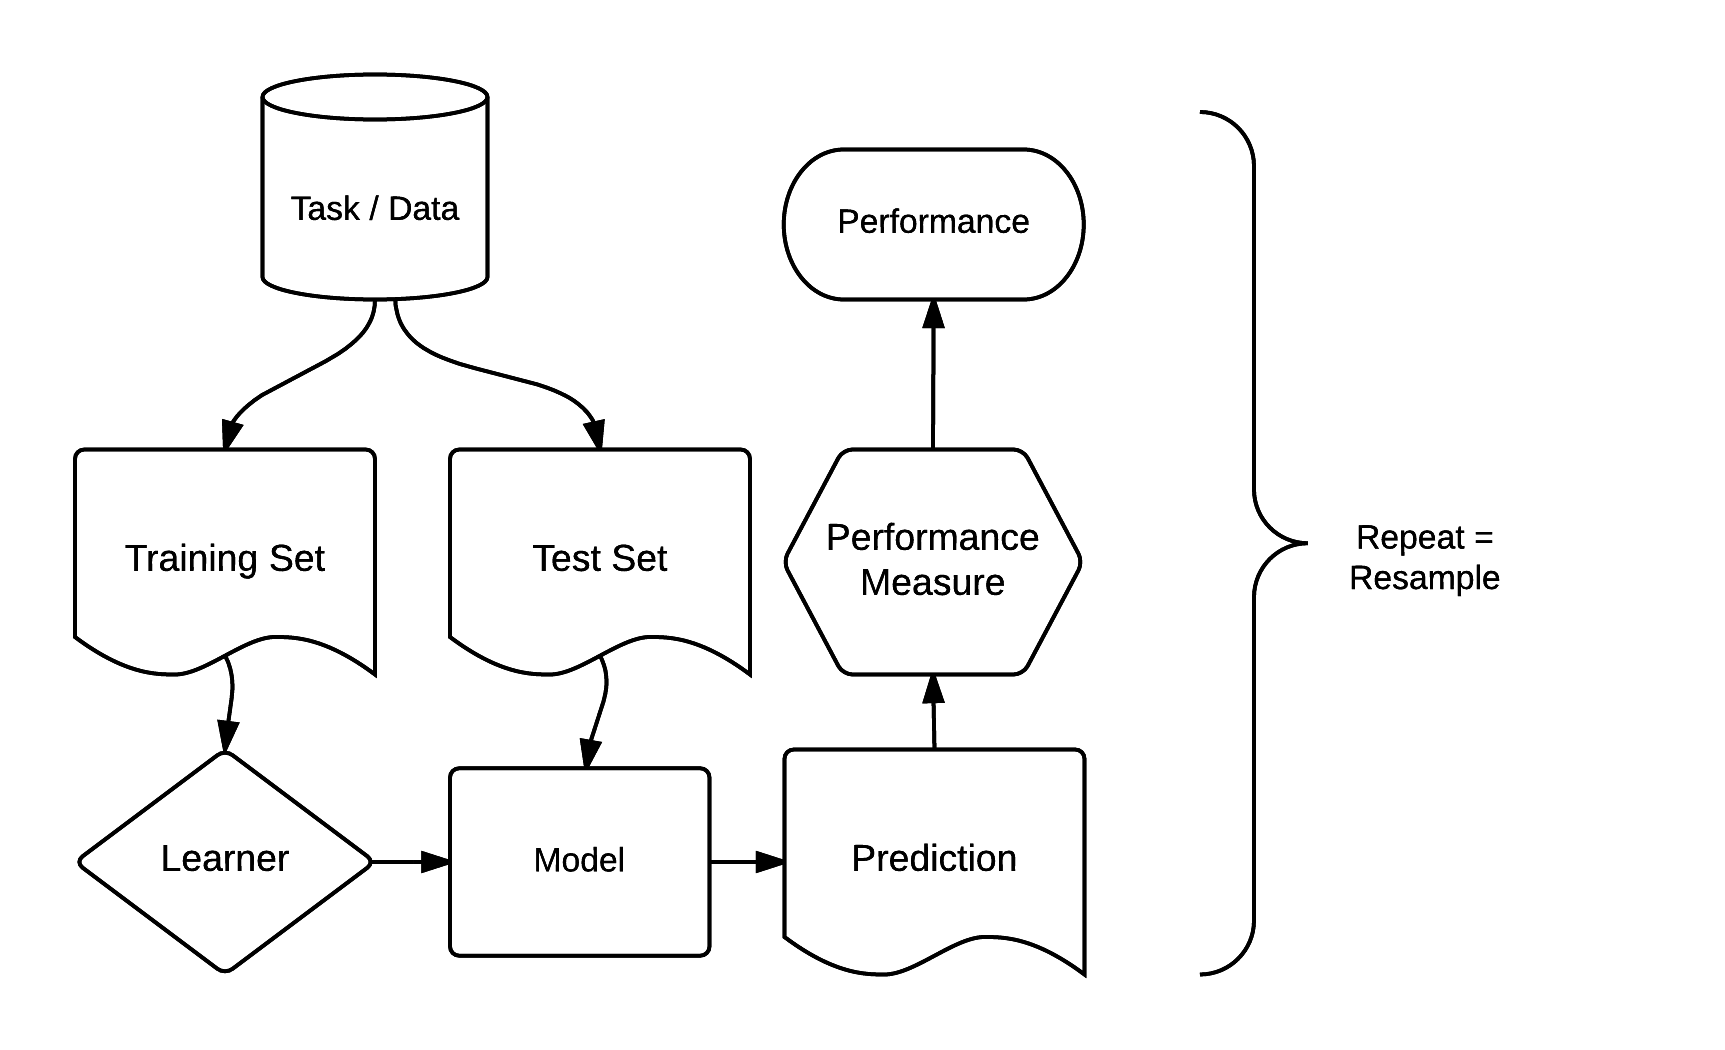
\includegraphics[width=\textwidth]{img/ml_abstraction.png}
						\end{myblock}
					}
				\end{minipage}
			\end{beamercolorbox}
		\end{column}
		\begin{column}{.245\textwidth}
			\begin{beamercolorbox}[center]{postercolumn}
				\begin{minipage}{.98\textwidth}
					\parbox[t][\columnheight]{\textwidth}{
						\begin{myblock}{Task}
							Tasks objects store data (\codeinline{backend}) and additional meta-data for machine learning problems.
							\\
							\begin{codebox}
								task = \textbf{TaskClassif}\$new(backend, target)
							\end{codebox}
							For classification, \codeinline{target} is a character vector with representing class labels.
							\\
							\begin{codebox}
								task = \textbf{TaskRegr}\$new(backend, target)
							\end{codebox}
							For regression, \codeinline{target} is a numeric vector.
							\\
							\begin{codebox}
								task = \textbf{tsk}(.key)
							\end{codebox}
							Get predefined task by \codeinline{.key}.
							\\
							\begin{codebox}
								task\$\textbf{select}(cols)
							\end{codebox}
							Subsets the task based on feature names (\codeinline{cols}).
							\\
							\begin{codebox}
								task\$\textbf{filter}(rows)
							\end{codebox}
							Subsets the task based on row ids (\codeinline{rows}).
						\end{myblock}
						\begin{myblock}{Learner}
						Learner objects provide a unified interface to machine learning algorithms. The \href{https://github.com/mlr-org/mlr3learners}{mlr3learners package} (https://github.com/mlr-org/mlr3learners) and the \href{https://github.com/mlr3learners}{mlr3learners organization} (https://github.com/mlr3learners) provide additional learning algorithms for mlr3.
						\\
						\begin{codebox}
							learner = \textbf{lrn}(.key, ...)
						\end{codebox}
						Get learner by \codeinline{.key} and construct the learner with specific hyperparameter and settings (...) in one go.
						\\
						\begin{codebox}
							learner\$\textbf{param\_set}
						\end{codebox}
						Returns a description of hyperparameter settings.
					\end{myblock}
						\vfill
					}
				\end{minipage}
			\end{beamercolorbox}
		\end{column}
		\begin{column}{.245\textwidth}
			\begin{beamercolorbox}[center]{postercolumn}
				\begin{minipage}{.98\textwidth}
					\parbox[t][\columnheight]{\textwidth}{
						\begin{myblock}{Train \& Predict}
							Training fits a model to a given task.
							\\
							\begin{codebox}
								learner\$\textbf{train}(task, row\_ids)
							\end{codebox}
							Train model on the observations in \codeinline{task} with \codeinline{row\_ids}.
							\\
							\begin{codebox}
								prediction = learner\$\textbf{predict}(task, row\_ids)
							\end{codebox}
							Predict on the observations in \codeinline{task} with \codeinline{row\_ids}.
							\\
							\begin{codebox}
								measure = \textbf{msr}(.key)
							\end{codebox}
							Get measure by \codeinline{.key}.
							\\
							\begin{codebox}
								prediction\$\textbf{score}(measure)
							\end{codebox}
							Access performance with \codeinline{measure}.
						\end{myblock}
						\begin{myblock}{Resampling}	
						Resampling objects define how a task is partitioned into a series of train and test sets. mlr3 entails six predefined resampling strategies:
						\\
						\begin{itemize}
							\item \codeinline{holdout} - Holdout-validation.
							\item Leave-one-out cross validation.
							\item \codeinline{cv} - Cross-validation.
							\item \codeinline{repeated\_cv} - Repeated cross-validation.
							\item \codeinline{bootstrap} - Out-of-bag bootstrap.
							\item Monte-Carlo cross-validation.
						\end{itemize}
						\vspace{0.5cm}
						Keys to access resampling strategies.
						\\
						\begin{codebox}
							resampling = \textbf{rsmp}(.key)
						\end{codebox}
						Get resampling strategy by \codeinline{.key}.
						\\
						\begin{codebox}
							resampling\$\textbf{instantiate}(task)
						\end{codebox}
						Apply resampling strategy on \codeinline{task}.
					\end{myblock}
					}
				\end{minipage}
			\end{beamercolorbox}
		\end{column}
		\begin{column}{.245\textwidth}
			\begin{beamercolorbox}[center]{postercolumn}
				\begin{minipage}{.98\textwidth}
					\parbox[t][\columnheight]{\textwidth}{
						\begin{myblock}{Resample \& Benchmark}
							The \codeinline{resample} function uses the series of train and test sets defined by the \codeinline{Resampling} object to estimate the performance of a learning algorithm. For this, a model is fitted on each train set (\codeinline{\$train}) and the performance is estimated on the corresponding test sets (\codeinline{\$predict}).
							\\
							\begin{codebox}
								rr = \textbf{resample}(task, learner, resampling)
							\end{codebox}
							Executes resampling and returns a \codeinline{ResampleResult} object.
							\\
							\begin{codebox}
								rr\$\textbf{aggregate}(measure)
							\end{codebox}
							Calculate the average performance with \codeinline{measure}.
							\\
							\begin{codebox}
								rr\$\textbf{score}(measure)
							\end{codebox}
							Extract the performance of individual resampling iterations with \codeinline{measure}.
							\\
							\\
							The \codeinline{benchmark} function is used to compare the performance of different learners on multiple task and/or different resampling schemes.
							\\
							\begin{codeboxmultiline}[width=21.95cm]
								design = \textbf{benchmark\_grid}(\\
								\hspace*{1ex}task = tsks(.keys),\\
								\hspace*{1ex}learner = lrns(.keys),\\
								\hspace*{1ex}resampling = rsmps(.keys)))
							\end{codeboxmultiline}
							\codeinline{benchmark\_grid} creates an exhaustive design and instantiates the resampling.
							\\
							\begin{codebox}
								bmr = \textbf{benchmark}(design)
							\end{codebox}
							Execute benchmark with \codeinline{design}. \\
							
							Returns a \codeinline{\robotomono{BenckmarkResult}} object:
							\\
							\begin{codeboxmultiline}[width=27cm]
								\scriptsize{
								<BenchmarkResult> of 404 rows with 8 resampling runs\\
								nr task\_id \space\space\space\space learner\_id resampling\_id iters warnings errors\\
								1 \space\space\space sonar \space classif.rpart 
								\space\space\space\space\space\space holdout 
								\space\space\space\space 1 
								\space\space\space\space\space\space\space 0 
								\space\space\space\space\space 0\\
								2 \space\space\space sonar \space classif.rpart 
								\space\space repeated\_cv 
								\space\space 100
								\space\space\space\space\space\space\space 0
								\space\space\space\space\space 0\\
								3 \space\space\space sonar classif.ranger
								\space\space\space\space\space\space holdout
								\space\space\space\space 1
								\space\space\space\space\space\space\space 0
								\space\space\space\space\space 0\\
								4 \space\space\space sonar classif.ranger
								\space\space repeated\_cv
								\space\space 100
								\space\space\space\space\space\space\space 0
								\space\space\space\space\space 0\\
								5 \space\space\space\space spam  
								\space classif.rpart
								\space\space\space\space\space\space holdout
								\space\space\space\space 1
								\space\space\space\space\space\space\space 0
								\space\space\space\space\space 0\\
								6 \space\space\space\space spam 
								\space  classif.rpart
								\space\space repeated\_cv
								\space\space 100
								\space\space\space\space\space\space\space 0
								\space\space\space\space\space 0\\
								7 \space\space\space\space spam 
								classif.ranger
								\space\space\space\space\space\space holdout
								\space\space\space\space 1
								\space\space\space\space\space\space\space 0 
								\space\space\space\space\space 0\\
								8 \space\space\space\space spam
								classif.ranger
								\space\space repeated\_cv
								\space\space 100
								\space\space\space\space\space\space\space 0
								\space\space\space\space\space 0
							}
						\end{codeboxmultiline}
					    \vspace{1cm}
					    \begin{codebox}
					    	bmr\$\textbf{aggregate}(measure)
					    \end{codebox}
					    Calculate and aggregate performance.
						\end{myblock}\vfill
					}
				\end{minipage}
			\end{beamercolorbox}
		\end{column}
	\end{columns}
\end{frame}
\end{document}
